\documentclass[12pt]{article}
\usepackage[utf8]{inputenc}
\usepackage{amssymb}
\usepackage[legalpaper, portrait, margin=0.8in]{geometry}
\usepackage{algorithm}
\usepackage{graphicx}
\usepackage{hyperref}

\title{Homework 5 - COT5405}
\author{Kobee Raveendran}
\date{December 2021}

\begin{document}
    \maketitle

    \begin{enumerate}
        \item \textbf{Suppose you have an undirected graph with only positive integer edge weights. How can you use BFS to find 
        the length of the shortest path from a source vertex to every other vertex in $O((E+V)D)$ time, where $D$ is the 
        maximum weight on an edge.}

        Since BFS is usually only useful for unweighted graphs (or graphs that have uniform edge weights), we can't apply 
        it outright here. What we could instead do is ``expand'' all the weights. Since all edge weights here are 
        positive integers, I'll say the ``default'' weight is 1. Thus, all edges with weight not equal to 1 will have 
        to be expanded into a series of edges with weight 1. So, for example, an edge with weight 7 would be split up 
        into 7 edges each with weight 1 (also with dummy vertices between these edges). Once we've done this for all the 
        original edges, we can then run BFS as normal to find the shortest path lengths.

        The only extra work we incur here is from splitting up all the edges with weights not equal to 1. This is a 
        process bounded by the weight of the maximum edge in the graph, which we know here is $D$. Thus, for all $|E|$ edges, we incur at 
        most $D$ work per edge, and since inserting an edge means also inserting a vertex, for all vertices we also incur 
        this $D$ work per vertex. So, our final runtime is $O(|E|D + |V|D) = O((|E| + |V|)D)$.

        \item \textbf{Consider a directed weighted graph with non-negative edge weights. For some cases, it is necessary 
        to compute the length of the shortest path from every vertex $v$ to a target vertex $t$. Describe how you can 
        compute this in the same time complexity as in Dijkstra's algorithm.}

        This problem seems like an inversion of the goal of Dijkstra's algorithm. To solve it, we can set the 
        target vertex $t$ in this problem to be the ``source'' vertex in Dijkstra's algorithm. Then, we just run through 
        Dijkstra's algorithm to find the shortest paths from the ``source'' (our target $t$) to all other vertices. 
        Since we don't need to maintain the actual paths, we do not need to reverse them (we can just maintain the length 
        of the paths as we progress through). Since all we've done is run Dijkstra but swap the ``source'' and ``target'' 
        vertices, the runtime is exactly the same.

        \item \textbf{Consider a directed graph where each edge has some existence probability, i.e., say an edge $e$ 
        exists with probability $Pr(e)$, where $0 \leq Pr(e) \leq 1$. If a path from $u$ to $v$ has the edges 
        $e_1, e_2, ..., e_k, $ then the probability that the path exists is given by $Pr(e_1) \cdot Pr(e_2) \cdot ... 
        \cdot Pr(e_k)$. Given a source vertex $s$ and a target vertex $t$, describe how you can use Dijkstra's algorithm 
        to find a path from $s$ to $t$ that has the maximum probability of existing.}

        To obtain the maximum probability of a path existing, we should first try to maximize the probabilities of the 
        constituent edges along the path, which will maximize their product. So, we should essentially be flipping another goal of 
        Dijkstra's algorithm (which originally aims to find the shortest paths, but here we want the ``longest'' path in 
        that the path's edge weights should be maximized rather than minimized). However, I don't believe Dijkstra's can be used 
        to find longest paths outright, but we can try converting our problem from edge maximization to edge minimization. 
        To do that, I'll use a trick from optimization commonly seen in machine learning loss function optimization, which is 
        to seek to minimize the negative log likelihood instead of maximizing the regular likelihood. All we have to do is, for all edges 
        in the graph, set the edge weight $w_{edge}$ to $w_{edge} = -\log w_{edge}$.

        We've now converted our maximization problem into a minimization one. If you aren't familiar with the negative 
        log likelihood trick, to convince yourself that this works, see the graph of $-\log x$ in figure 
        \ref{fig:negative-log-likelihood} below. Note how, in the range $[0, 1]$ (where our original edge weight probabilities 
        lie), $-\log (x)$ is decreasing and non-negative as $x$ increases. For example, $-\log (0.6) \approx 0.221$ while $-\log (0.8) \approx 0.097$; 
        in other words, the higher probability has been converted into a smaller value. Since we are also dealing with logs, 
        we can replace the multiplication in the original problem with addition (so, the existence probability of a path 
        is now the sum of its edge weights rather than the product).
        
        Anyway, now that we have a minimization problem, we can just run Dijkstra's as normal on our updated graph and 
        find the ``shortest'' path (the smallest constituent edge weights along the path). This path is the path that 
        would yield the highest probability of existing in our original graph.

        To do all this, we just need $O(|E|)$ time to first update each edge weight $w$ to $-\log w$. Then we run 
        Dijkstra's as normal, which of course doesn't change its runtime.

        \begin{figure}[ht!]
            \begin{center}
                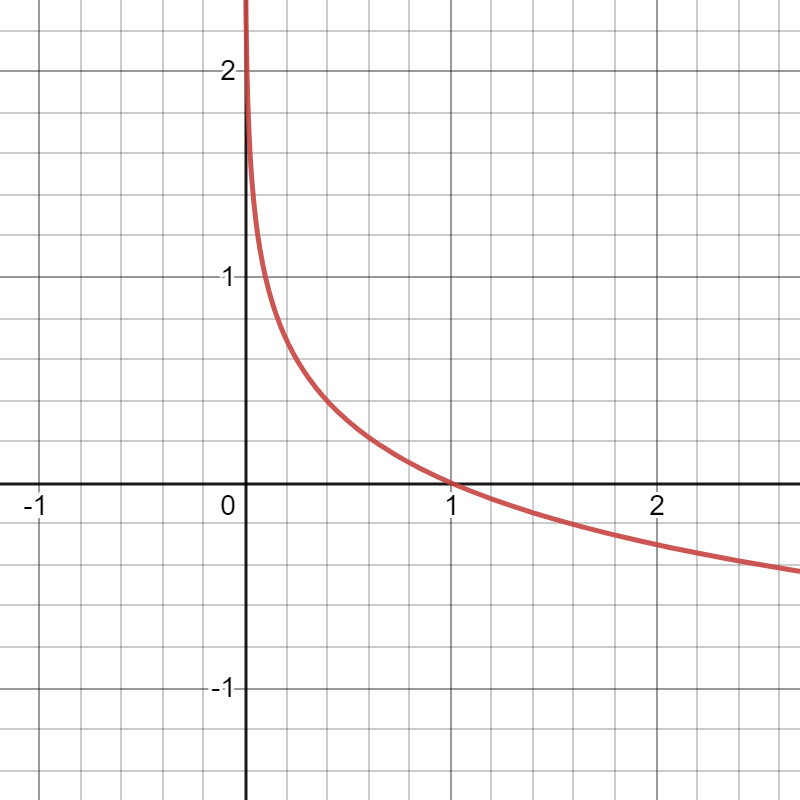
\includegraphics[scale = 0.35]{assets/negative_logx.png}
                \caption{Graph of $f(x) = -\log x$. Note that our original edge probabilities (the values on the 
                $x$-axis) are now mapped to a $y$-value on the curve. Also note that these $y$-values decrease from 
                $+\infty$ to 0 as the $x$-values increase from 0 to 1.}
                \label{fig:negative-log-likelihood}
            \end{center}
        \end{figure}

        \item \textbf{Given a directed acyclic graph, find the length of the longest path in the graph in $O(n+m)$ time. 
        Note that we are NOT looking for the longest path starting at a particular vertex, rather the overall longest 
        path that can start at any arbitrary vertex.}

        \textit{NOTE: Here I'm assuming the graph is unweighted. If it is actually weighted, then we could possibly try 
        another approach like negating the edge weights, then finding the shortest paths in this new graph.}

        In a DAG, we can find the longest path (and its length) starting at a vertex $v$ using a DFS from that vertex. However, since we 
        want the overall longest path, we'd have to run a DFS for all vertices, which would give us a quadratic runtime 
        ($O(n^2)$, where $n = |V| +  |E|$).

        However, we can notice that these longest paths build upon each other and have an optimal substructure property, 
        allowing us to use DP. For example, to get the length of the longest path from a node at one end of a graph to the other end, 
        we need only add the length from that node to a central node and the length from that central node to a node 
        at the opposite end of the graph.

        In our DP matrix, the length of the longest path from all vertices will be initialized to 0. Then, iterating 
        over the set of vertices, we assign \texttt{dp[v]} to be the max over all of its neighbors lengths (plus 1) and 
        its own value (\texttt{dp[v]}). 
        
        In other words, \texttt{dp[v] = max(max(dp[$n_i$] for $n_i$ in neighbors) + 1, dp[v])}. Once \\
        we've run through this for all vertices, we need only scan through \texttt{dp} one final time and take the 
        maximum value, which is our final answer. We are not doing any repeated work, and so in our loop over all 
        $|V|$ vertices, we will just encounter all $|V|$ vertices and $|E|$ edges, giving us a total runtime of 
        $O(|V| + |E|)$, or $O(n + m)$ as per the problem statement (using linear extra space for the DP table).

    \end{enumerate}
\end{document}